\documentclass{article}
\usepackage[margin=1in]{geometry}
\usepackage{fancyhdr}
\usepackage{indentfirst}
\usepackage{graphicx}
\usepackage{subfigure}
\usepackage{subfigmat}
\usepackage{bm, amssymb, amsmath, array, pdfpages}
\usepackage{listings}

\usepackage{titlesec}

\graphicspath{{Figures/}}

% define some commands to maintain consistency
 \newcommand{\pkg}[1]{\texttt{#1}}
 \newcommand{\cls}[1]{\textsf{#1}}
 \newcommand{\file}[1]{\texttt{#1}}
\newcommand{\todo}[1]{\textcolor{red}{[TODO: #1]}}
\newcommand{\adgremark}[1]{\textcolor{blue}{[ADG: #1]}}
\newcommand{\R}{\mathbb{R}}
\newcommand{\CLmax}{{C_L}_\text{max}}
\newcommand{\LDmax}{L/D_\text{max}}
\newcommand{\alphamax}{\alpha_\text{max}}
\def\ip<#1,#2>{\left\langle #1,#2\right\rangle}

%%%%%%%%%%%%%%%%%%%%%%%%%%%%%%%%%%%%%%%%%%%%%%%%%%%%%%%%%%
% MODIFICATIONS TO ALLOW HEADER ON THE TITLE PAGE
%%%%%%%%%%%%%%%%%%%%%%%%%%%%%%%%%%%%%%%%%%%%%%%%%%%%%%%%%%

\makeatletter
% Copied from article.cls
\renewcommand\maketitle{\par
  \begingroup
    \renewcommand\thefootnote{\@fnsymbol\c@footnote}%
    \def\@makefnmark{\rlap{\@textsuperscript{\normalfont\@thefnmark}}}%
    \long\def\@makefntext##1{\parindent 1em\noindent
            \hb@xt@1.8em{%
                \hss\@textsuperscript{\normalfont\@thefnmark}}##1}%
    \if@twocolumn
      \ifnum \col@number=\@ne
        \@maketitle
      \else
        \twocolumn[\@maketitle]%
      \fi
    \else
      \newpage
      \global\@topnum\z@   % Prevents figures from going at top of page.
      \@maketitle
    \fi
    \thispagestyle{fancy}\@thanks % was {empty}
  \endgroup
  \setcounter{footnote}{0}%
  \global\let\thanks\relax
  \global\let\maketitle\relax
  \global\let\@maketitle\relax
  \global\let\@thanks\@empty
  \global\let\@author\@empty
  %\global\let\@date\@empty
  \global\let\@title\@empty
  \global\let\title\relax
  \global\let\author\relax
  %\global\let\date\relax
  \global\let\and\relax
}
% end of copy
\makeatother

\newcommand*{\vertbar}{\rule[1ex]{0.5pt}{2.5ex}}
\newcommand*{\horzbar}{\rule[.5ex]{2.5ex}{0.5pt}}

%%%%%%%%%%%%%%%%%%%%%%%%%%%%%%%%%%%%%%%%%%%%%%%%%%%%%%%%%%
% TITLE, DATE, AUTHOR, HEADERS
%%%%%%%%%%%%%%%%%%%%%%%%%%%%%%%%%%%%%%%%%%%%%%%%%%%%%%%%%%


\begin{document}
\pagestyle{fancy}
\lhead{\textit{\bf Notes: A Lagrangian Spray Model for Airfoil Icing}}
\rhead{\bf February 2015} %empty
\title{\LARGE \bf
Notes: A Lagrangian Spray Model for Airfoil Icing}
\author{Anthony DeGennaro}
\date{July 2014}
\maketitle

%%%%%%%%%%%%%%%%%%%%%%%%%%%%%%%%%%%%%%%%%%%%%%%%%%%%%%%%%%
% ANTHONY DEGENNARO'S PROPOSAL
%%%%%%%%%%%%%%%%%%%%%%%%%%%%%%%%%%%%%%%%%%%%%%%%%%%%%%%%%%

\section{Introduction and Motivation}
The purpose of these notes is to describe the ongoing development of a wing ice accretion code 
which applies techniques from the liquid spray community to improve on existing methods.

It is well-known that individual droplets in the air can significantly affect ice accretion on wings.
As an example, an ATR-72 crashed in Roselawn, Indiana in 1994; it is speculated that this incident 
was largely due to Supercooled-Liquid Droplets (SLDs) in the air. This crash has led to a revamping 
of the FAA regulations on flight conditions to explicitly consider freezing drizzle/rain.

Existing computational codes for icing generally do {\it not} track each individual droplet impinging 
on the wing throughout the course of a simulation. The reason for this is simple: there are too many 
droplets for this to be computationally feasible. We can demonstrate this easily with a back of the 
envelope calculation: assuming the liquid water content (LWC) of the air to be 0.3 g/m$^3$, the 
airspeed to be 100 m/s, and the mean volumetric diameter (MVD) of the liquid droplets to be 50 $\mu$m, 
this gives a free-stream flux of about 500 million particles per square meter per second. Since wing icing 
simulations can frequently last 5-10 minutes or longer, one is faced with the proposition of tracking (potentially)
billions of particles over the course of one simulation (this is not even accounting for new droplets created 
through the process of droplet splashing and breakup).

Existing methods deal with this problem in a few ways. First, many methods do not employ a Lagrangian 
approach; rather, they treat the liquid/air as a two-phase continuum and use Eulerian formulations, which 
automatically circumvents the need to track all particles. Regardless, most methods assume that the 
liquid mass impinging on the wing surface can be modeled as a continuum (the so-called ``collection 
efficiency"). Because of this assumption, there is no need to advect the billions of particles one would 
do in a fully time-resolved Lagrangian simulation; instead, one need only advect an initial ``sheet" of 
particles, observe how that sheet impinges on the wing surface, and calculate a mass flux ratio that way. 
Of course, another notable assumption here is that the collection efficiency does not vary over the 
course of the simulation, even though the droplet properties may be randomly distributed.

Both of these solutions lead to fast simulations at the expense of ignoring (1) the statistical effect of 
having droplet properties which are randomly distributed and (2) the effect on the ice shape of individual 
droplets. This is where we hope to make a contribution. Borrowing from methods used in the spray 
community, we formulate the icing problem probabilistically, by equipping the freestream droplet 
properties with a probability density function. We then formulate a Lagrangian in which the advected 
particles are actually ``clumps" of droplets. This keeps the number of parcels tracked in each simulation 
relatively low. In order to investigate the statistical effects of the droplet distribution, one need only generate 
a multirealization ensemble of simulations. We also hope to develop a thermodynamic model that governs the 
behavior of the individual droplets as they impinge and freeze on the surface; this would potentially help 
towards investigating the effect of individual droplets on ice shape.

\newpage
\section{Probabilistic Framework}
We begin our approach with a probabilistic framework governing the distribution of droplet properties. 
Specifically, we assume that the number density of droplets may be written as a function of the droplet 
properties: $f({\bf x}, {\bf u}, R, e; t)$. Here, ${\bf x}$ denotes position, ${\bf u}$ velocity, $R$ radius, $e$ 
energy, and $t$ time. If we define $N$ as the number of droplets, then:
\begin{equation}
\label{dN}
dN(t_0) = f({\bf x_0}, {\bf u_0}, R_0, e_0; t_0) \; dV
\end{equation}
gives the average number of droplets 
located inside an infinitesimal hypervolume $dV$ about the location $({\bf x_0}, {\bf u_0}, R_0, e_0; t_0)$ 
(here, average is meant in the sense of the mean over a multirealization ensemble). Hence, $f$ is a 
distribution function, whose integral gives the number of droplets in a hypervolume of parameter space:
\begin{equation}
N_{V}(t_0) = \int_{V} f({\bf x}, {\bf u}, R, e; t_0) \; d{\bf x} \; d{\bf u} \; dR \; de
\end{equation}
Similarly, the droplet number density at some location and time ${\bf x_0}, t_0$ is given by the integral:
\begin{equation}
n({\bf x_0}, t_0) = \int f({\bf x_0}, {\bf u}, R, e; t_0) \; d{\bf u} \; dR \; de
\end{equation}
We may obtain ensemble average properties as moments of our distribution function; for any droplet 
property $\phi$, we have:
\begin{equation}
\overline{\phi({\bf x_0},t_0)} = \frac{1}{n({\bf x_0}, t_0)} \int \phi \; f \; d{\bf u} \; dR \; de 
\end{equation}

\section{Sampling Technique}
We now describe a method for generating realizations from $f$. Clearly, it is impractical to do a ``straightforward"
Monte Carlo sampling of $f$, since this would generate a prohibitively large number of droplets. Instead, we can do 
the following. Consider a finite number $M$ samples of the distribution space. For each of these locations, we may 
approximate the local number of droplets in a small volume centered at that location from Eq.(\ref{dN}). Note that, 
for fine resolution, this number may be less than unity; for coarse resolution, it may be much greater than unity. 

At each location, any variation in the state values is presumed to be small within the small volume, and so we collapse 
any local uncertainty in the state values into a delta function, and conserve local mass by 
simply creating a certain number of identical particles, giving rise to what are effectively particle ``clumps". 
To be explicit, consider a computational domain consisting of 
an airfoil and its grid. Droplets will enter this computational domain by appearing at different times inside a domain 
of injection $V$, which is fixed in space. Conservation of total mass for all time in the injection domain gives:
\begin{equation}
\label{mass}
\sum_i^M N_i m_i = \int_V \left(\frac{4}{3} \pi \rho R^3\right) f dV dt
\end{equation}
And, from Eq.(\ref{dN}), we approximate the number of local particles as:
\begin{equation}
\label{number}
N_k({\bf X}_k,t) \approx f({\bf X}_k,t) \Delta V
\end{equation}
Where, for brevity, ${\bf X}_k = ({\bf x}_k, {\bf u}_k, R_k, e_k)$ denotes the vector of droplet properties at some time at sample $k$.
We can now solve for the volume size $\Delta V$ from Eq.(\ref{mass}-\ref{number}), giving:
\begin{equation}
\Delta V = \left. \int_V \left(\frac{4}{3} \pi \rho R^3\right) f dV dt \middle/ \sum_i^M f({\bf X}_i) m_i \right.
\end{equation}

\section{Advection Method}
If we neglect shattering or coalescence of droplets, then the droplet numbers are conserved (both the total number 
and the local number of particles at each of the $M$ sample locations). We can state conservation of local 
droplet numbers in each of our sample locations by $M$ conservation equations:
\begin{equation}
\frac{\partial N_i}{\partial t} + \nabla_{\bf X} \cdot \left(\dot {\bf X} N_i \right) = 0 \; \; \; , \;\;\; i=1...M
\end{equation}
These partial differential equations are hyperbolic, and their trajectories govern the paths of our particle clumps.
The trajectories may be found by solving for the characteristics, which closely resemble a Lagrangian method on individual droplets:
\begin{equation}
\begin{aligned}
\dot{\bf x}_i & = {\bf u}_i  \\
\dot{\bf u}_i & = \sum_j \frac{1}{m_i} {\bf F_j}_i \\
\dot{R}_i & = -\frac{\dot{m}_i}{4 \pi \rho R_i^2} \\
\dot{e}_i & = \frac{\dot{m}_i}{m_i} \left( e_i - e_{\text{surf}} + \frac{\dot{q}_i}{\dot{m}_i}\right) + \frac{B_i}{\rho}
\end{aligned}
\end{equation}
where ${\bf F_j}_i$ represents the $j^{th}$ force on the droplet associated with parcel $i$, $\dot{m}_i$ is the mass loss 
in a parcel due to evaporation, $e_{\text{surf}}$ is the internal energy of the liquid on the surface of impingement, 
$\dot{q_i}$ is the heat loss due to evaporization, and $B_i$ represents energy flux to the volume occupied by the liquid if gas filled 
that volume.

So, the method described here for advecting a distribution of particles is technically a method of characteristics approach 
to a multicontinua formulation (where each of the continua are represented by the individual ``chunks" of droplets); it is, strictly 
speaking, not a Lagrangian discrete particle method.

\section{Examples}
Here we briefly show some examples on sampling a particle distribution as described earlier. The first step involves formulating 
the actual distribution function $f({\bf X},t)$. Here, we make the reasonable assumption that $f({\bf X},t)$ can be written as the 
product of several independent distributions: 
\begin{equation}
f({\bf X},t) = f_{{\bf x}}({\bf x})f_{{\bf u}}({\bf u})f_R(R)f_e(e)f_t(t)
\end{equation}
We are free to construct our distribution function in any way we choose, and so, for simplicity, we 
assume in this example that the droplets are distributed uniformly in space and time, and normally in velocity, radius, and 
energy. We also assume that the distributions separately integrate in the following way:
\begin{equation}
\begin{aligned}
\int f_{\bf x}({\bf x}) d{\bf x} & = N_{\mathcal{D}}  \\
\int f_{\bf t}(t) dt & = \left. T_{\text{sim}} \middle/ \Delta t_{\mathcal{D}} \right. \\
\int f_{\bf{u}}({\bf u}) d{\bf u} = \int f_R(R) dR = \int f_e(e) de & = 1
\end{aligned}
\end{equation}
where $N_{\mathcal{D}}$ is the average number of droplets in the injection domain $\mathcal{D}$ at any time, $T_{\text{sim}}$ 
is the duration of the simulation, and $\Delta t_{\mathcal{D}}$ is the average time it takes for a droplet to traverse 
the entire injection domain $\mathcal{D}$. This way, our expression for the average number of droplets in the entire simulation 
nicely turns out to be:
\begin{equation}
N_{\text{sim}} = \int f({\bf X},t) d{\bf X} dt = N_{\mathcal{D}} T_{\text{sim}}/\Delta t_{\mathcal{D}}
\end{equation}
which is just the product of the average number of particles in the injection domain at any point in time and how many times (on average) 
the entire injection domain empties and must be completely refilled.

We determine the injection domain by calculating the impingement limits for a particle which is of average size at two different 
locations upstream of the airfoil. This ensures that most of the parcels we advect will actually impinge on the airfoil. $\Delta t_{\mathcal{D}}$ 
can be estimated as the length of the injection domain divided by the freestream velocity. The average number of particles in 
$\mathcal{D}$ can be estimated from the Liquid Water Content (LWC) of the air.

If we set LWC = $0.4$ g/m$^3$, the freestream velocity to $U = 100$ m/s, the average droplet radius to $\overline{R} = 50 \; \mu$m, and the 
length of the simulation to $T_{\text{sim}} = 10$ minutes, then the total number of droplets is $N_{\text{sim}} \approx 450,000$. 

Below, we 
show the cumulative distribution of the number of droplets per parcel assuming several different desired numbers of parcels. We also 
show the resulting statistics of a sample realization in each case. As one can clearly see, there is a trade-off between resolution of the 
statistics of the realization, and the number of parcels one has to track. It is also clear that as the number of parcels is increased towards 
the total number of droplets in the simulation, all parcels converge toward having a single droplet each, and this method becomes a 
regular Lagrangian Monte Carlo method.
\begin{figure}
\centering
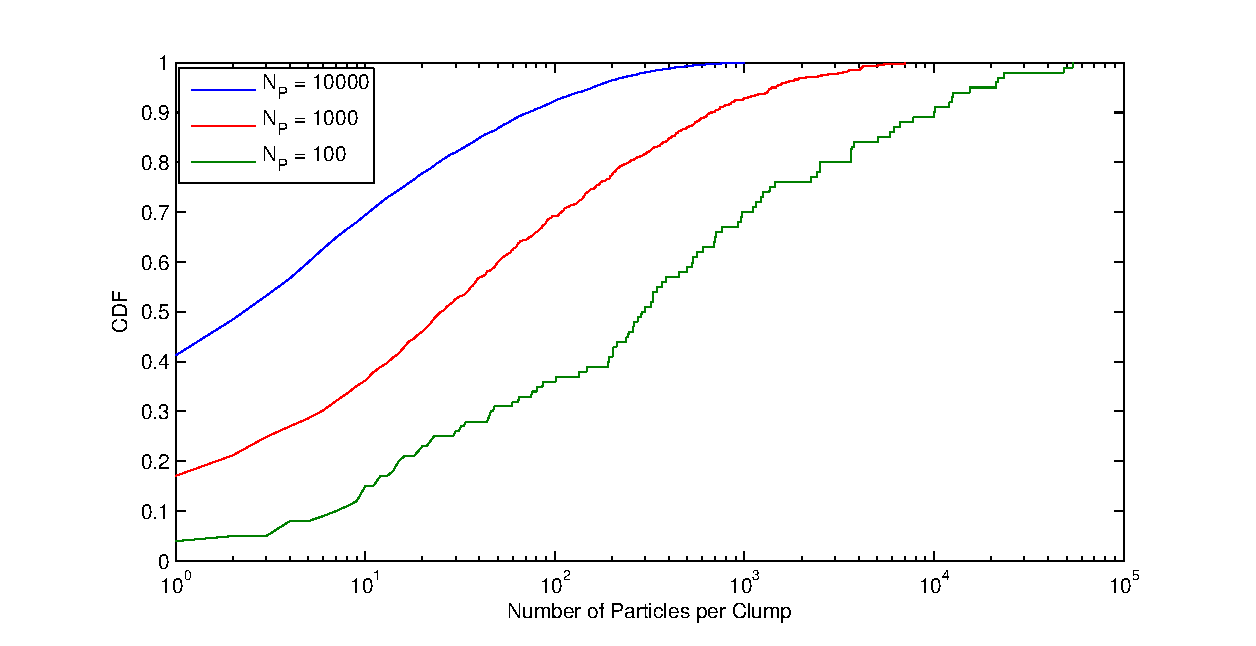
\includegraphics[width=.5\textwidth] {CDFClump.eps}
\caption{CDF for the number of droplets per parcel for $M$ = 100, 1000, 10000.}
\end{figure}











\end{document}